\begin{figure*}[!ht]
	\centering
	%
	\subfigure[IP trace1]{
		\begin{minipage}[t]{0.255\textwidth}{
		\prefig
		\begin{center}
		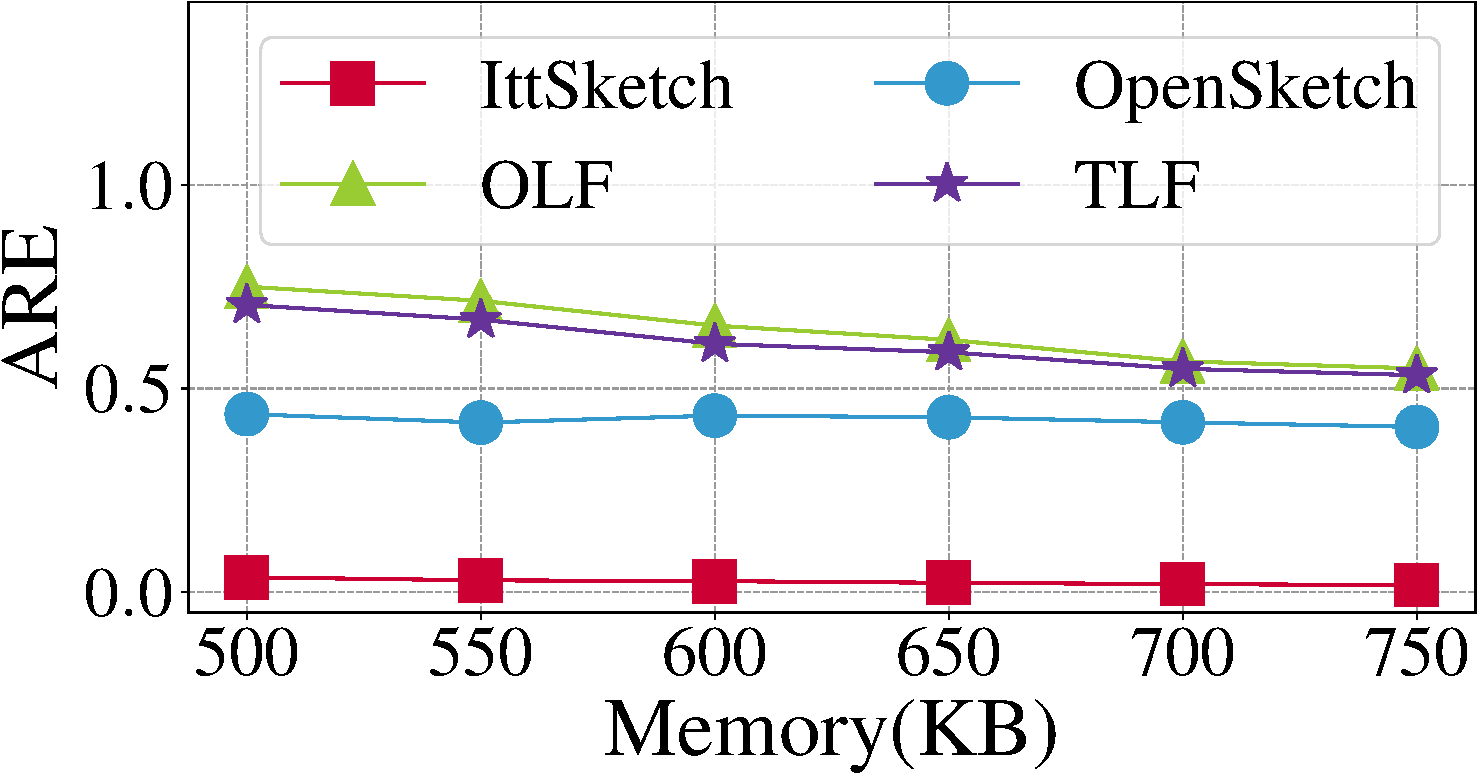
\includegraphics[width=0.95\textwidth, ]{Figures/sup/sup_are/_sup_ip_are.pdf}
		\end{center}
		}
		\postfig
		\adjustfigs
		\prefigcaption
		\label{sup_are_ip}
		\postfigcaption
		\end{minipage}
	}
	%
	\subfigure[IP trace2]{
		\begin{minipage}[t]{0.23\textwidth}{
		\prefig
		\begin{center}		
		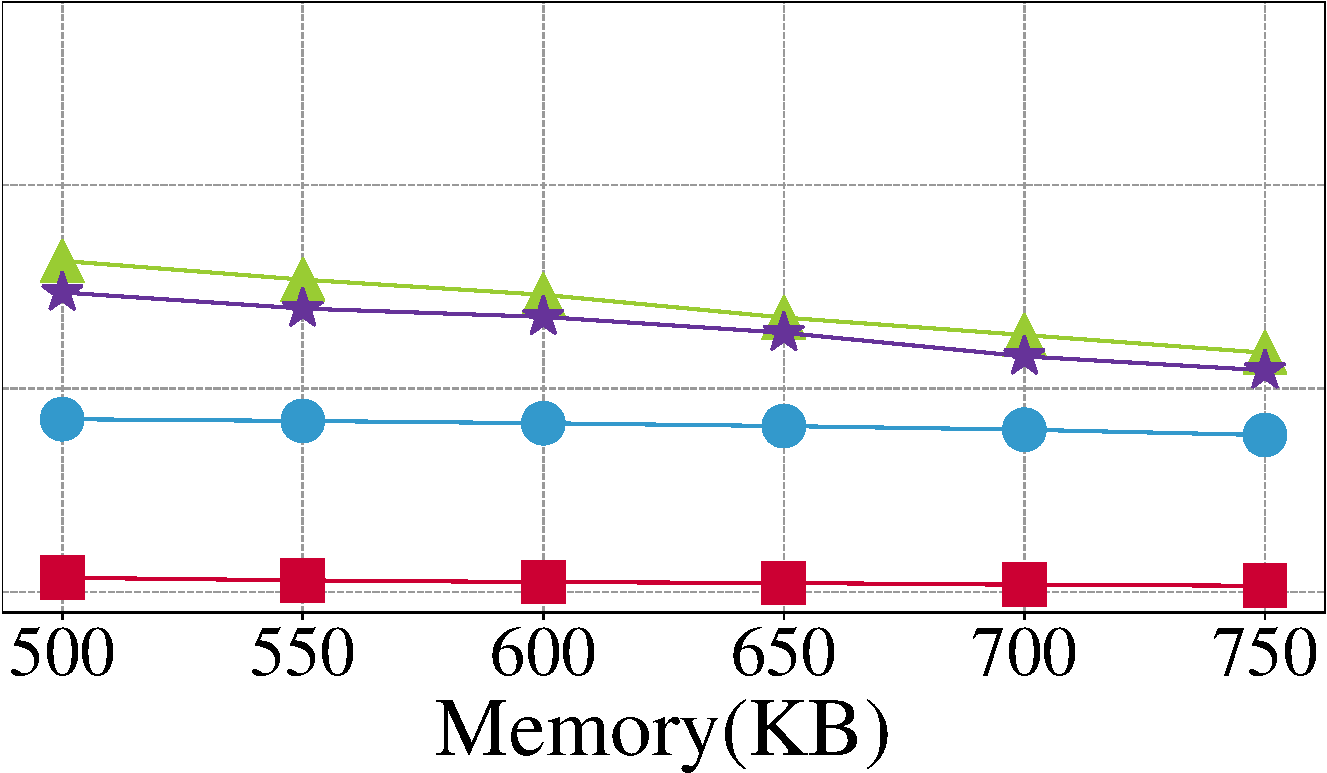
\includegraphics[width=0.95\textwidth, ]{Figures/sup/sup_are/_sup_ip4_are.pdf}
		\end{center}
		}
		\postfig 
		\adjustfigs
		\prefigcaption
		\label{sup_are_ip4}
		\postfigcaption
		\end{minipage}
	}
	%
	\subfigure[IP trace3]{
		\begin{minipage}[t]{0.23\textwidth}{
		\prefig
		\begin{center}		
		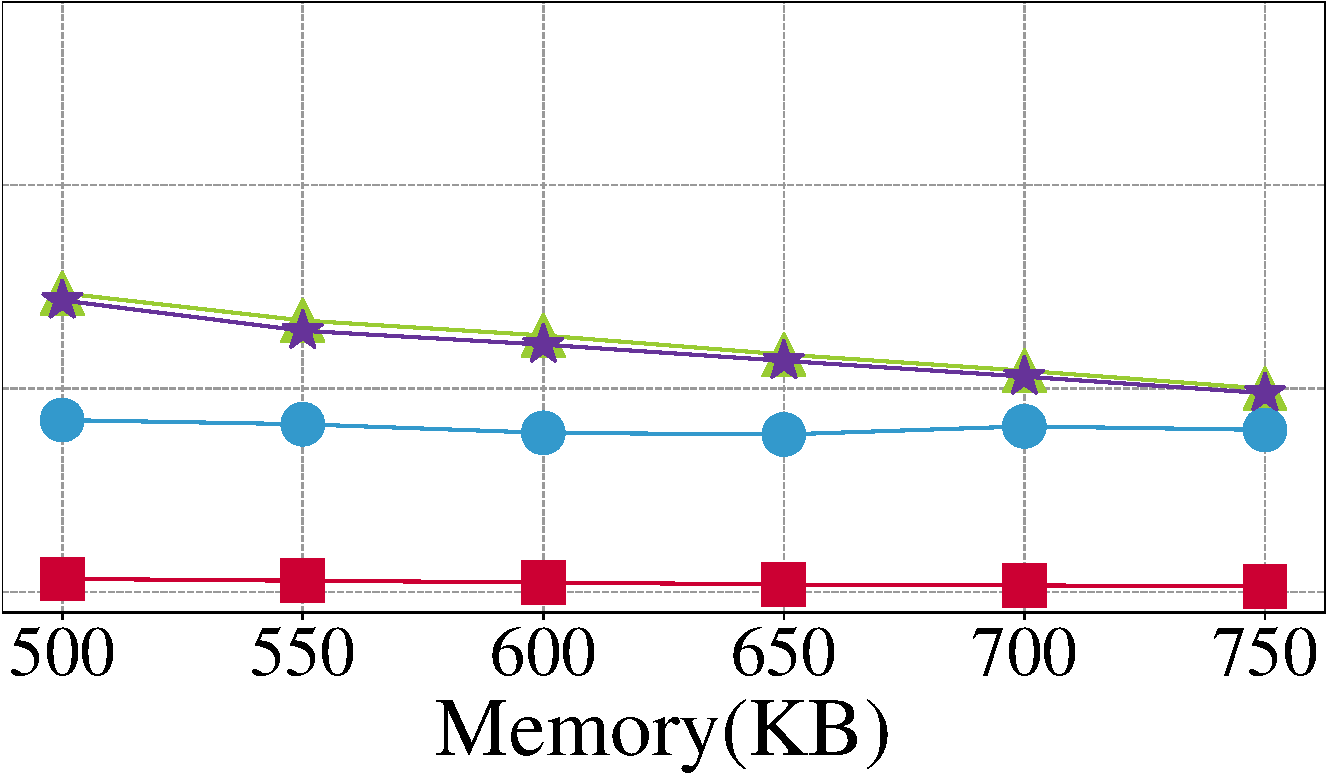
\includegraphics[width=0.95\textwidth, ]{Figures/sup/sup_are/_sup_ip6_are.pdf}
		\end{center}
		}
		\postfig 
		\adjustfigs
		\prefigcaption
		\label{sup_are_ip6}
		\postfigcaption
		\end{minipage}
	}
	%
	\subfigure[IP trace4]{
	    \begin{minipage}[t]{0.23\textwidth}{
		\prefig
		\begin{center}
		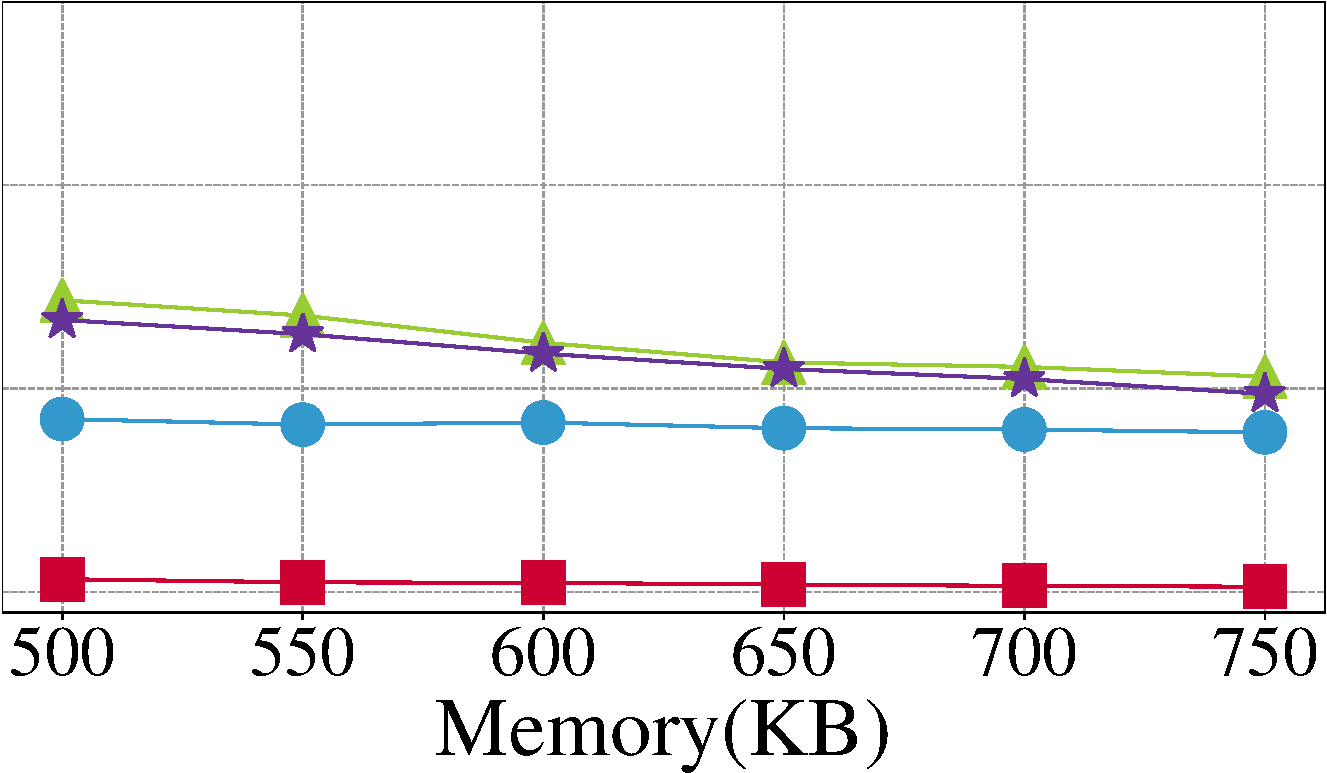
\includegraphics[width=0.95\textwidth, ]{Figures/sup/sup_are/_sup_ip8_are.pdf}
		\end{center}
		}
		\postfig 
		\adjustfigs
		\prefigcaption
		\label{sup_are_ip8}
		\postfigcaption
		\end{minipage}
	}
	%
	\vvv \vvv
    \caption{ARE of finding \tasktwo.}
	\label{sup_are}
\end{figure*}


\begin{figure*}[!ht]
	\centering
	%
	\subfigure[IP trace1]{
		\begin{minipage}[t]{0.255\textwidth}{
		\prefig
		\begin{center}
		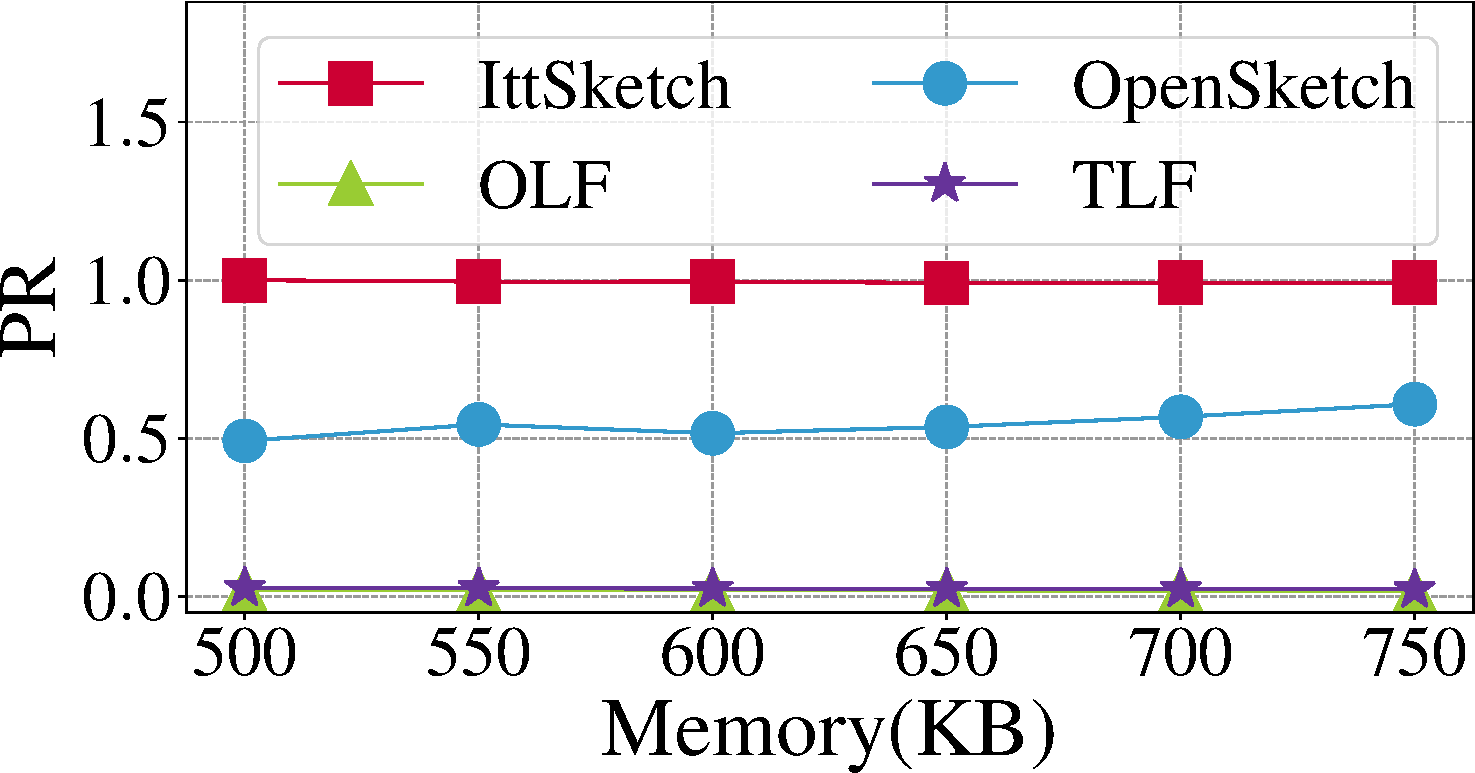
\includegraphics[width=0.95\textwidth, ]{Figures/sup/sup_pr/_sup_ip_pr.pdf}
		\end{center}
		}
		\postfig
		\adjustfigs
		\prefigcaption
		\label{sup_pr_ip}
		\postfigcaption
		\end{minipage}
	}
	%
	\subfigure[IP trace2]{
		\begin{minipage}[t]{0.23\textwidth}{
		\prefig
		\begin{center}		
		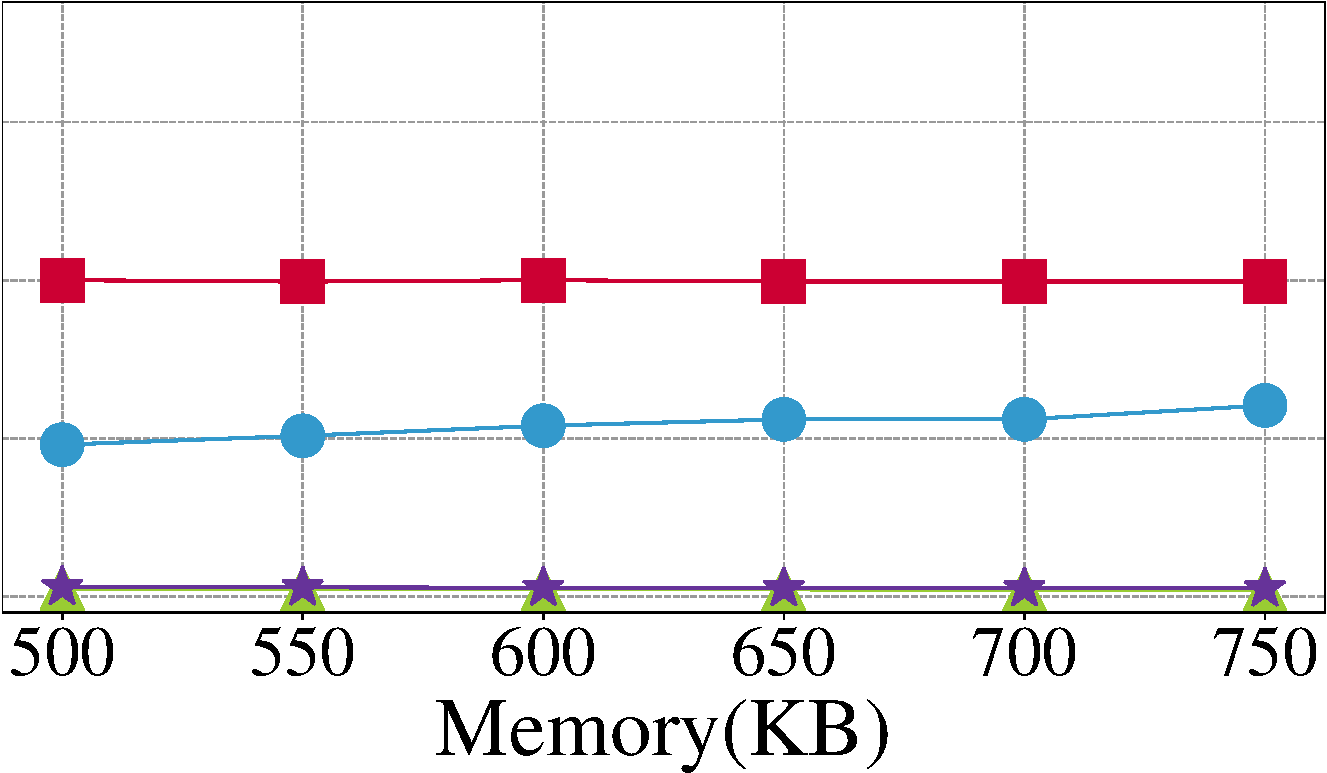
\includegraphics[width=0.95\textwidth, ]{Figures/sup/sup_pr/_sup_ip4_pr.pdf}
		\end{center}
		}
		\postfig 
		\adjustfigs
		\prefigcaption
		\label{sup_pr_ip4}
		\postfigcaption
		\end{minipage}
	}
	%
	\subfigure[IP trace3]{
		\begin{minipage}[t]{0.23\textwidth}{
		\prefig
		\begin{center}		
		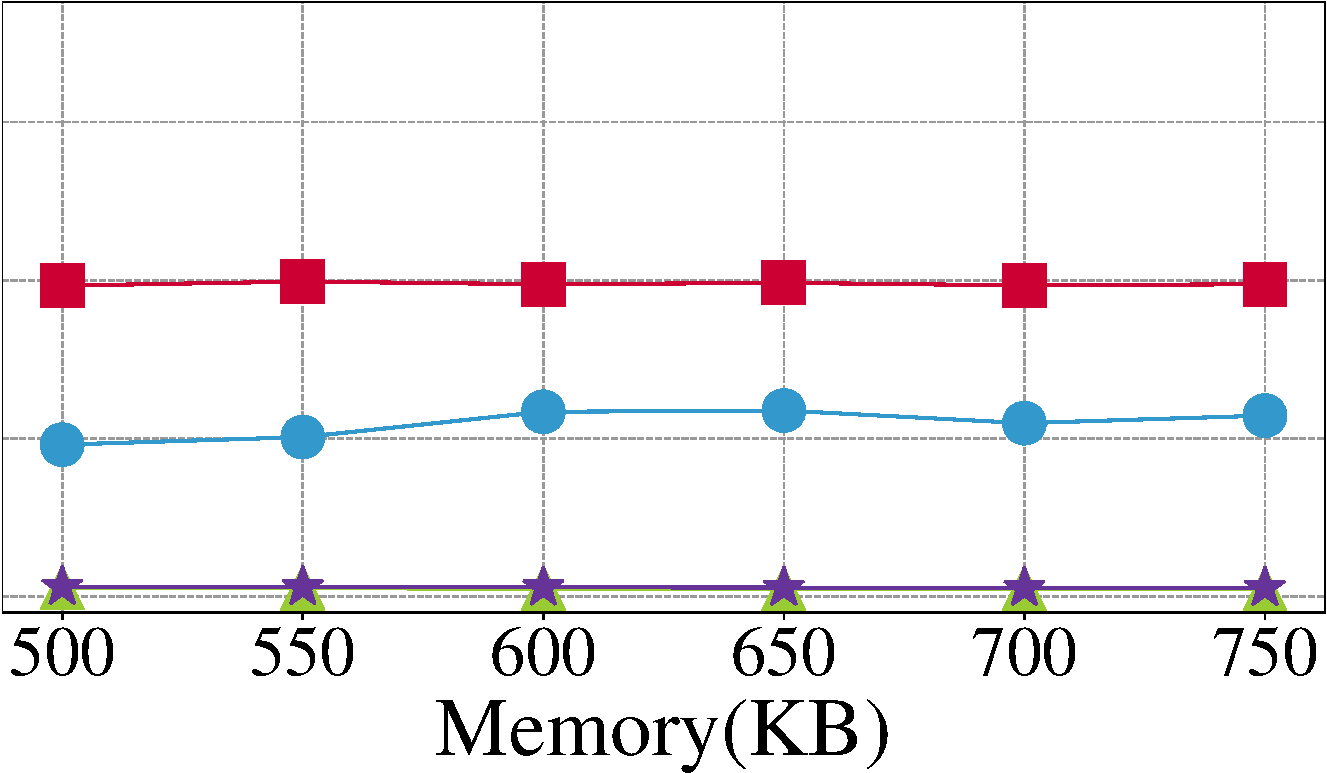
\includegraphics[width=0.95\textwidth, ]{Figures/sup/sup_pr/_sup_ip6_pr.pdf}
		\end{center}
		}
		\postfig 
		\adjustfigs
		\prefigcaption
		\label{sup_pr_ip6}
		\postfigcaption
		\end{minipage}
	}
	%
	\subfigure[IP trace4]{
		\begin{minipage}[t]{0.23\textwidth}{
		\prefig
		\begin{center}
		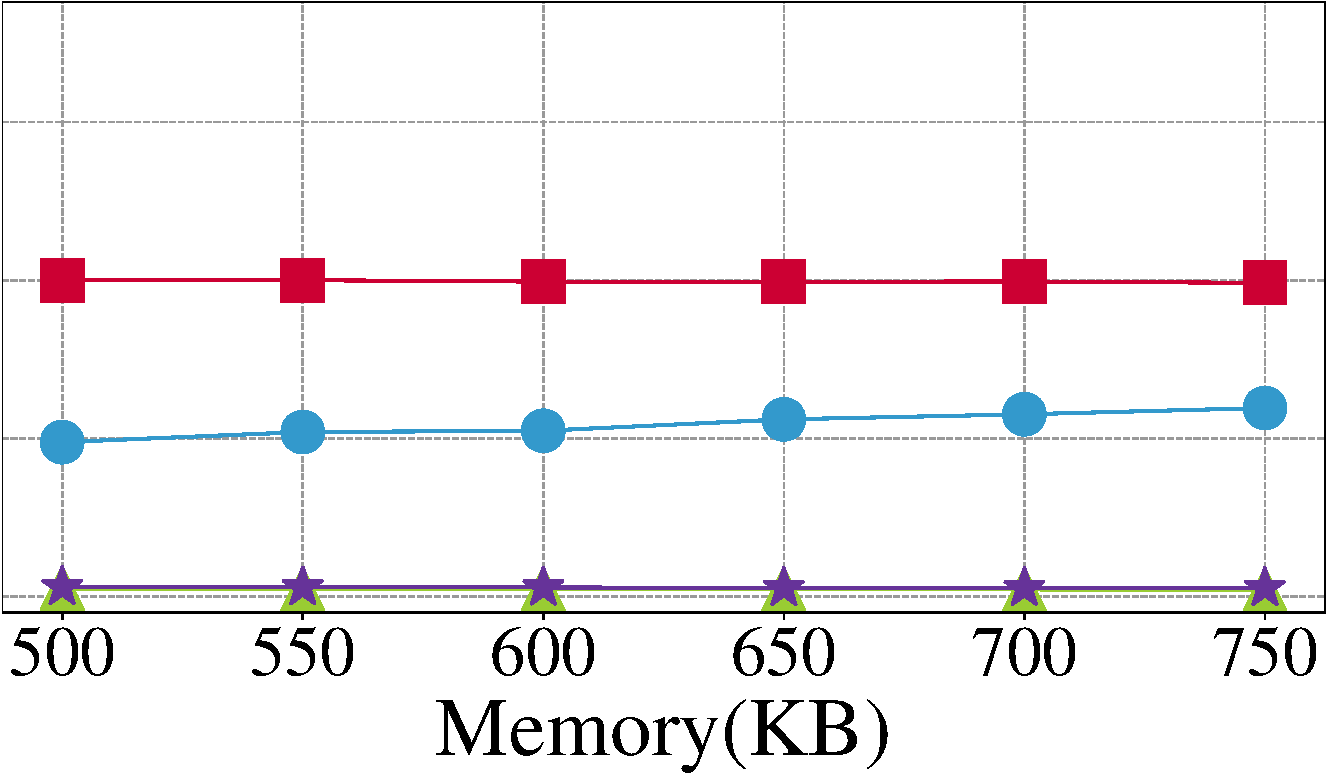
\includegraphics[width=0.95\textwidth, ]{Figures/sup/sup_pr/_sup_ip8_pr.pdf}
		\end{center}
		}
		\postfig 
		\adjustfigs
		\prefigcaption
		\label{sup_pr_ip8}
		\postfigcaption
		\end{minipage}
	}
	%
	\vvv \vvv
    \caption{PR of finding \tasktwo.}
	\label{sup_pr}
\end{figure*}

\begin{figure*}[!ht]
	\centering
	%
	\subfigure[IP trace1]{
		\begin{minipage}[t]{0.247\textwidth}{
		\prefig
		\begin{center}
		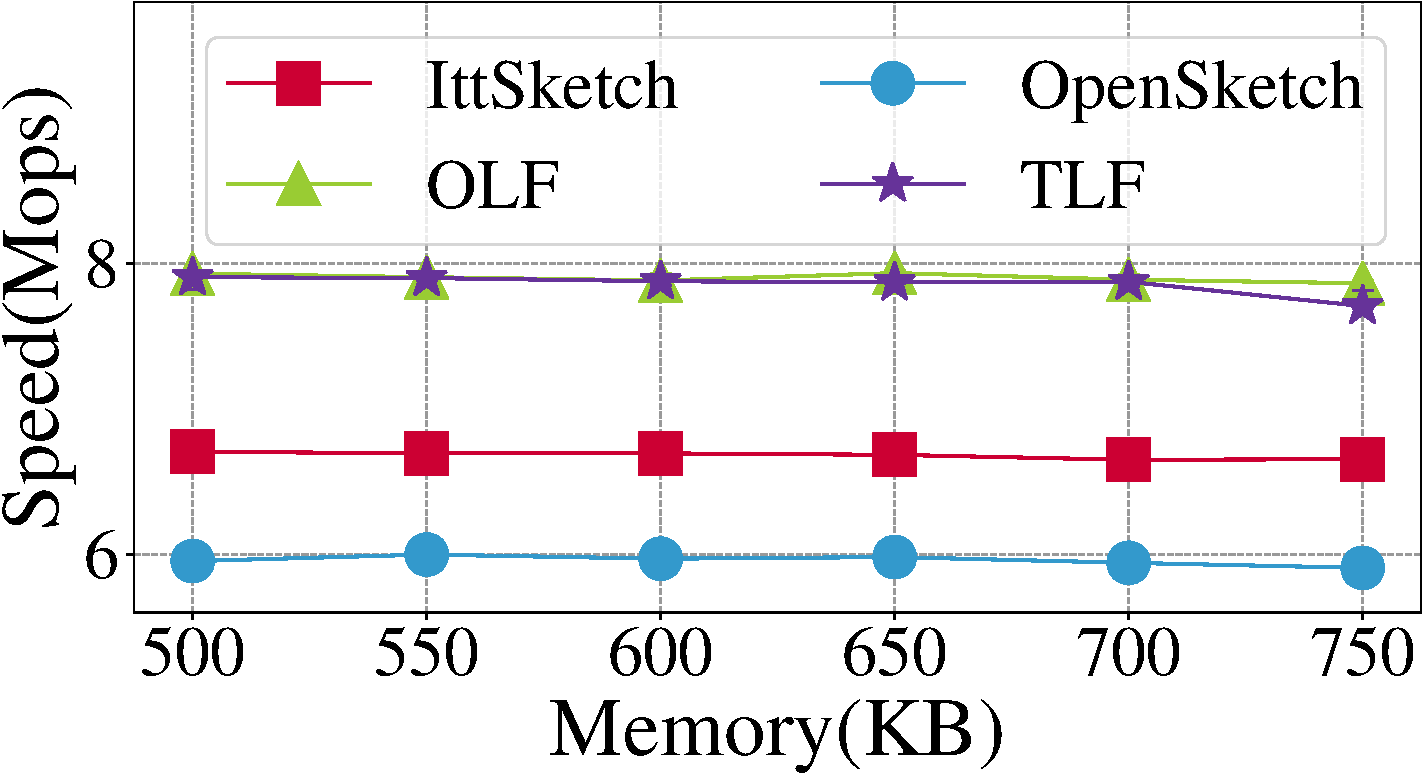
\includegraphics[width=0.95\textwidth, ]{Figures/sup/sup_speed/_sup_ip_speed.pdf}
	    \end{center}
	    }
		\postfig
		\adjustfigs
		\prefigcaption
		\label{sup_speed_ip}
		\postfigcaption
		\end{minipage}
	}
	%
	\subfigure[IP trace2]{
		\begin{minipage}[t]{0.23\textwidth}{				\prefig
		\begin{center}		
		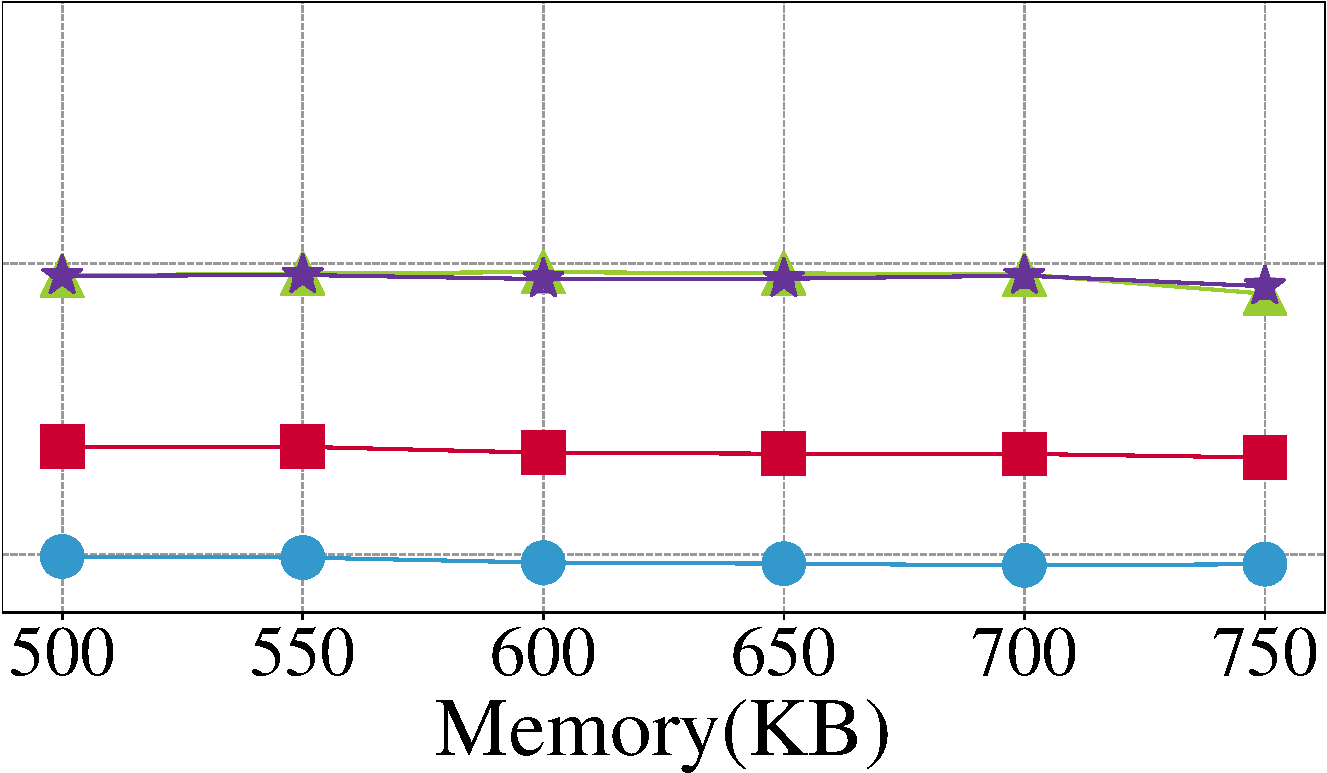
\includegraphics[width=0.95\textwidth, ]{Figures/sup/sup_speed/_sup_ip4_speed.pdf}
		\end{center}
		}
		\postfig 
		\adjustfigs
		\prefigcaption
		\label{sup_speed_ip4}
		\postfigcaption
		\end{minipage}
	}
	%
	\subfigure[IP trace3]{
		\begin{minipage}[t]{0.23\textwidth}{
		\prefig
		\begin{center}		
		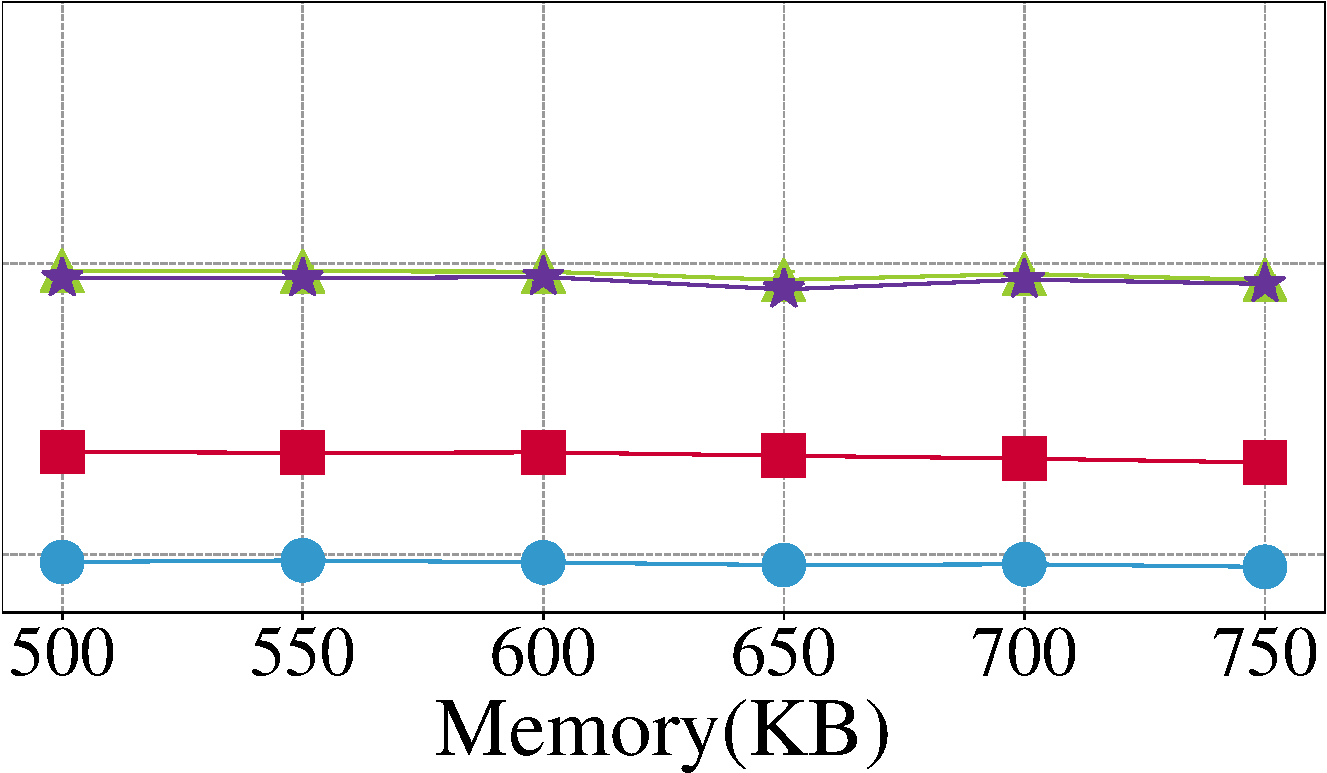
\includegraphics[width=0.95\textwidth, ]{Figures/sup/sup_speed/_sup_ip6_speed.pdf}
		\end{center}
		}
		\postfig 
		\adjustfigs
		\prefigcaption
		\label{sup_speed_ip6}
		\postfigcaption
		\end{minipage}
	}
	%
	\subfigure[IP trace4]{
		\begin{minipage}[t]{0.23\textwidth}{
		\prefig
		\begin{center}
		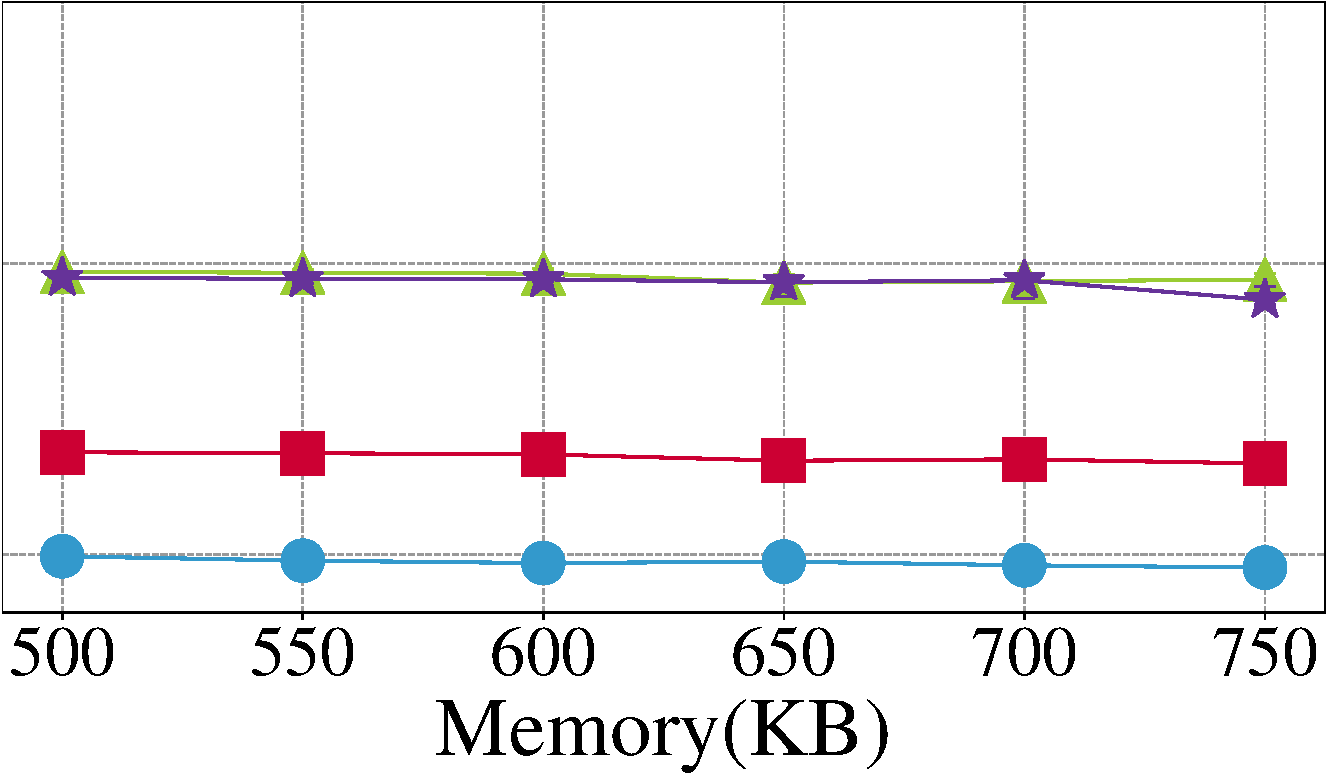
\includegraphics[width=0.95\textwidth, ]{Figures/sup/sup_speed/_sup_ip8_speed.pdf}
		\end{center}
		}
		\postfig 
		\adjustfigs
		\prefigcaption
		\label{sup_speed_ip8}
		\postfigcaption
		\end{minipage}
	}
	%
	\vvv \vvv
    \caption{Speed of finding \tasktwo.}
	\label{sup_speed}
\end{figure*}

%\presub
\subsection{Evaluation on Finding \taskfour} %\postsub
\label{eva_four}

\noindent\textbf{Parameter Setting:}
%We compare three frameworks: \sketchname, \EHname and \Splittername. For each frameworks, we using CM Sketch, CM-CU Sketch and Count Sketch approaches.
%
%We compare 5 approaches: CM \sketchname, CM-CU \sketchname, Count \sketchname, \EHname {} and \Splittername.
We compare 3 algorithms: \sketchname, \chafr\cite{flowradar}, and \chafrcf\cite{coldfilter}.
For \chafr{} and \chafrcf, the parameters are set according to the recommendation of the authors.
In the experiments, we compare PR, CR, and the insertion speed among the 3 algorithms. We vary the amount of memory from from 2MB to 4.5MB. We choose this range because \chafr{} cannot report any heavy changes if memory size is smaller. Also, we set the memory size of \sketchname{} to $1/20$ of the memory size of the other algorithms when we compare PR and CR. The reason for this is that when memory is larger than 2MB, the CR and PR of \sketchname{} are 1. 
%To compare these algorithms more conveniently, we reduce the memory size of \sketchname.


\noindent\textbf{PR (Figure~\ref{cha_pr_syn}-\ref{cha_pr_net}):}
We find that on three real-world datasets, the PR of \sketchname{} is around 4.1 times and 3.6 times higher than \chafr{} and \chafrcf. 
On the synthetic dataset, the PR of \chafr{} is 0 when its memory size is less than 2.5 MB. The PR of \sketchname{} is around 6.2 times higher than \chafrcf. 
			
			
\noindent\textbf{Speed (Figure~\ref{cha_speed_syn}-\ref{cha_speed_net}):}
We find that the insertion speed of \sketchname{} is around 2.1 times and 3 times faster than \chafr{} and \chafrcf{} on three real-world datasets and one synthetic dataset.

\noindent\textbf{CR (Figure~\ref{cha_cr_syn}-\ref{cha_cr_net}) in Appendix \ref{app:fig}:}
We find that, on three real-world datasets, the CR of \sketchname{} is around 64 times and 35 times higher than \chafr{} and \chafrcf. 
On the synthetic dataset, the CR of \chafr{} is 0 when its memory size is less than 2.5 MB. The CR of \sketchname{} is around 16 times higher than \chafrcf. 


\noindent\textbf{Summary:}
%
1) Although the memory size of \sketchname{} is only $1/20$ of other algorithms, the CR of \sketchname{} is often more than 0.98 when its memory size is more than 0.98 on three real-world datasets and one synthetic dataset. 
% Steve: broken sentence, please fix it.
In contrast, the CR of \chafr{} is often lower than 0.2 because it will decode few items if the memory size is too small.

2) The PR of \sketchname{} is lower than the PR of \sketchname~ in other datasets, for there are less differences between the two periods in the synthetic dataset. Therefore, we have to spend more space on finding heavy changes in the synthetic dataset. However, \sketchname{} still performs much better than \chafr{} and \chafrcf.